\documentclass[10pt]{amsart}
\usepackage[a4paper,margin=1in]{geometry}
\usepackage[T1]{fontenc}
\usepackage{lmodern,microtype,amssymb,graphicx,booktabs,placeins}
\usepackage{tikz}
\usetikzlibrary{arrows.meta}
\usepackage[hidelinks]{hyperref}

% the encodings of the figure set
\definecolor{bfS}{HTML}{0072B2}
\definecolor{bfR}{HTML}{D55E00}
\colorlet{bfblack}{black!17}

\numberwithin{equation}{section}
\newtheorem{theorem}[equation]{Theorem}
\newtheorem{proposition}[equation]{Proposition}
\newtheorem{lemma}[equation]{Lemma}
\theoremstyle{definition}
\newtheorem{definition}[equation]{Definition}
\newtheorem{example}[equation]{Example}
\theoremstyle{remark}
\newtheorem{remark}[equation]{Remark}

\newcommand{\T}{T}
\newcommand{\eps}{\varepsilon}
\newcommand{\FIG}{../figures/}
\newcommand{\bal}{\operatorname{bal}}
\setlength{\emergencystretch}{2em}

\title[Barnette's conjecture]{Barnette's conjecture in the dual triangulation}
\subjclass[2020]{05C45, 05C10, 05C70}
\date{14 November 2026}

\begin{document}
\begin{abstract}
A spanning subgraph in which every vertex has degree two need not be a single cycle.
We explain OpenAI's proof that every cubic, bipartite, 3-connected planar graph has a Hamiltonian cycle avoiding any given edge, working in the dual triangulation, where such a cycle is an acyclic set of edges containing exactly one side of every triangle.
The set is built from a choice of one corner in each black triangle, provided the sides opposite the chosen corners form a forest with one corner of the outer triangle in each tree.
A signed count of pairs of corner choices that differ in every triangle cancels the pairs whose opposite sides contain a cycle, while heights at the white triangles show that the count is not zero.
A prescribed edge lets the construction pass across separating triangles.
\end{abstract}
\maketitle

\section{Introduction}

A Hamiltonian cycle is a connected spanning subgraph in which every vertex has degree two.
In a cubic graph the degree condition is the easy half.
Deleting a perfect matching leaves every vertex with two edges, and a cubic bipartite graph has a perfect matching by Hall's theorem.
Connectivity is the whole problem.
On the cube, the two opposite squares form a subgraph of degree two with two components (Figure~\ref{fig:cube}(a)).

\begin{theorem}[OpenAI {\cite[Theorem~1.1 and Corollary~7.1]{openai2026}}]\label{thm:main}
Let $G$ be a finite simple graph that is cubic, bipartite, planar and $3$-connected, and let $e$ be an edge of $G$.
Then $G$ has a Hamiltonian cycle that does not contain $e$.
\end{theorem}

Here $3$-connected means that $G$ has at least four vertices and stays connected after deleting any two of them.
Barnette's conjecture is the case without $e$.
The edge $e$ is there for the induction of Section~\ref{sec:glue}, which cuts $G$ into smaller graphs and needs their cycles to agree on the cut.
That the version with $e$ is equivalent to the conjecture goes back to Kelmans, as explained by Hertel \cite[Corollary~3]{hertel2005} and by Gorsky, Steiner and Wiederrecht \cite[Theorem~4.3]{gsw2023}.

\subsection*{The plan}
We work in the dual triangulation $\T$ of $G$, whose triangles are coloured black and white by the two classes of $G$ (Figure~\ref{fig:cube}(b)).
A perfect matching of $G$ is a set of edges of $\T$ containing exactly one side of every triangle, and its complement in $G$ is a single cycle exactly when this set has no cycle (Section~\ref{sec:picture}).
Fix a black triangle $t_0$ containing the edge $e_0$ of $\T$ that crosses $e$.
Such an acyclic set chooses, in every other black triangle, one corner, and uses every vertex off $t_0$ exactly once; we call such a choice a \emph{state}.
Conversely a state $s$ yields an acyclic set whenever the sides opposite the chosen corners form a forest with one corner of $t_0$ in each tree (Section~\ref{sec:corners}, Figure~\ref{fig:cube}(d)--(f)).
A second state $r$ that differs from $s$ in every triangle orients these opposite sides and reduces the condition to ``no cycle''.
Counting such pairs with a sign, the pairs whose opposite sides contain a cycle cancel, and a regrouping by the cycles along which $r$ and $s$ differ (Figure~\ref{fig:cube}(c)) shows that the total is not zero as soon as one pair exists (Section~\ref{sec:pairs}).
A flow argument gives one pair when $\T$ has no separating triangle, that is, no triangle with vertices on both sides (Section~\ref{sec:flow}), and separating triangles are removed by cutting $\T$ into smaller triangulations whose solutions agree along the prescribed edge (Section~\ref{sec:glue}).

\begin{figure}[tb]
\centering
\includegraphics[width=0.78\textwidth]{\FIG 01-cube.pdf}
\caption{The whole construction on the cube, read along the rows. (a) A subgraph of degree two with two cycles. (b) The dual octahedron $\T$, black triangles shaded, with the outer face $t_0$ shown by the grey collar and its corners $0,1,2$ hollow. The prescribed side is $e_0=\{0,1\}$. (c) Two states, outlined $r$ and solid $s$, which differ in every black triangle; the arrows $r(t)\to s(t)$ form a cycle (Section~\ref{sec:pairs}). (d) The sides opposite the solid corners, dashed, form a forest with one root in each tree (Section~\ref{sec:corners}). (e) These sides and the two sides of $t_0$ other than $e_0$ form a spanning tree $S_s$ (bold); the dash-dotted tree joins the white faces across the remaining edges. (f) That tree selects one bold side in every face. The bold edges have no cycle, and the curve crossing all other edges is a Hamiltonian cycle of the cube.}
\label{fig:cube}
\end{figure}

\subsection*{History and sources}
Tait conjectured in 1884 that cubic $3$-connected planar graphs are Hamiltonian \cite{tait1884}, and Tutte disproved this in 1946 with a non-bipartite example \cite{tutte1946}.
Barnette asked whether bipartiteness rescues the statement \cite{barnette1969}.
Before 2026 the conjecture was known when all faces have four or six sides \cite{goodey1975}, under conditions on two of the three face colour classes \cite{feder-subi2006}, when all faces have at most eight sides \cite{schnieders2025}, and by computer up to 90 vertices \cite{hmm1985,bgm2021}.
In a preprint dated 24 September 2026, OpenAI proved Theorem~\ref{thm:main} \cite{openai2026}.
The objects of the proof are theirs: pairs of states, the opposite sides, the cycles along which two states differ, the disk identity, the cancellation for a fixed second state, the regrouping by cycles, the flow argument and the gluing.
States are the corner choices of Tutte's theory of trinity \cite{tutte1975}, see also \cite{hine-kalman2018}.
The target, two induced trees in $\T$, is Stein's reformulation \cite{stein1971} in the form of Alt, Payne, Schmidt and Wood \cite[Lemma~5]{apsw2016}.
Two expositions followed.
Li \cite{li2026} works in $G$ and replaces OpenAI's exponential sum by two sign-reversing involutions; his counts of crossings between half-rays from white vertices and matching edges are the same objects as the heights of Section~\ref{sec:pairs}.
An unsigned manuscript \cite{constructive2026} uses a real sign and an integer polynomial, describes partners by outdegrees, and gives an exact criterion for the existence of a pair and an enumeration algorithm.

Our account differs from \cite{openai2026} in four places, each proved in full below.
The disk identity is stated as ``one more white face than black'', with a short lemma that makes Euler's formula applicable to the inside of a cycle, and acyclicity of the final set is read off from it.
The sign of a pair is a product of local signs.
The weights are heights read along paths of faces, which are OpenAI's weights for one choice of their circulations; this removes the spokes, the sliding argument of \cite[Section~5.3]{openai2026} and the exponential sum.
The tree on the faces that selects the final set is obtained from the opposite sides by planar duality in $\T$; in $G$ it is Li's black dual trace \cite[Section~6]{li2026} with one extra leaf.

\subsection*{The example}
We follow one triangulation through every step (Figure~\ref{fig:dual}).
It has $13$ vertices, $22$ triangles and no separating triangle, and its dual $G$ has $22$ vertices.
It has $12$ states and $8$ pairs, all listed in Table~\ref{tab:pairs}.
Among them are a state whose opposite sides contain a cycle and two states that differ along a cycle enclosing three vertices.
The numbers quoted for the example come from exhaustive enumeration.

\section{The dual triangulation and the target}\label{sec:picture}

\subsection*{The dual}
Fix an embedding of $G$ in the sphere, with edges drawn as polygonal arcs.
Its dual $\T$ has a vertex in each face of $G$ and an edge crossing each edge of $G$ once.
Conversely $G$ is the graph of faces of $\T$: each face of $\T$ contains one vertex of $G$, and two faces are adjacent in $G$ when they share a side.

\begin{lemma}\label{lem:dual}
Let $G$ be as in Theorem~\ref{thm:main}.
Then $\T$ is a simple graph with at least four vertices, every face of $\T$ is bounded by a triangle, and the faces of $\T$ can be coloured black and white so that every edge of $\T$ has one black and one white face.
\end{lemma}

\begin{proof}
First, $G$ has no set of at most two edges whose removal separates a nonempty vertex set $U$ from the nonempty rest.
One vertex has three edges leaving it, and two vertices have at least four, since $G$ is simple.
So $|U|\ge3$, and likewise for the rest.
Deleting the at most two endpoints in $U$ of the cut edges leaves a nonempty part of $U$ with no edge to the rest, contradicting $3$-connectivity.

A loop of $\T$, or two edges of $\T$ joining the same two vertices, is a closed curve that meets $G$ in one or two points, on one or two edges of $G$.
The two ends of a crossed edge lie on opposite sides of the curve, so both sides contain vertices of $G$, and the crossed edges form a cut of size at most two.
Hence $\T$ is simple.
The face of $\T$ containing a vertex $v$ of $G$ is bounded by a closed walk through the three faces of $G$ at $v$, and in a simple graph a closed walk of length three is a triangle.
Euler's formula gives $|V(\T)|=|F(G)|=2+|E(G)|-|V(G)|=2+|V(G)|/2\ge4$.
Finally, colour the face of $\T$ containing $v$ by the class of $v$ in the bipartition of $G$.
The two faces at an edge of $\T$ contain the two ends of an edge of $G$, so they get different colours.
\end{proof}

From now on $\T$ is a \emph{coloured triangulation}: a simple graph with at least four vertices, embedded in the sphere so that every face is bounded by a triangle, with a black and white colouring of its faces in which every edge has one face of each colour.
Two faces share at most one side, since two faces with two common sides would have the same three corners, and that triangle would bound both of them, leaving no room for a fourth vertex.
The next lemma shows that $\T$ is connected.
We use it again for the inside of a cycle and for the pieces of Section~\ref{sec:glue}.

\begin{lemma}\label{lem:connected}
Let $R$ be a finite graph embedded in the sphere such that every face of $R$ is bounded by a cycle of $R$.
Then $R$ is connected.
\end{lemma}

\begin{proof}
Let $K$ be a component of $R$.
The boundary of a face is a cycle, which is connected, so it lies in one component.
Let $\Omega$ be the union of $K$ and the faces whose boundary lies in $K$, and $\Omega'$ the union of the other components and the other faces.
A point of $K$ has a neighbourhood that meets only $K$ and faces with that point on their boundary, and these faces have their boundary in $K$.
So $\Omega$ is open, and $\Omega'$ is open for the same reason.
They are disjoint, they cover the sphere, which is connected, and $\Omega$ is not empty.
Hence $\Omega'$ is empty and $R=K$.
\end{proof}

Each edge of $\T$ has exactly one black face and each black face has three sides, so the number of edges is three times the number of black faces, and likewise for white faces.
With Euler's formula this gives
\begin{equation}\label{eq:counts}
\#\{\text{black faces}\}=\#\{\text{white faces}\}=k,\qquad |E(\T)|=3k,\qquad |V(\T)|=k+2 .
\end{equation}
Figure~\ref{fig:dual} shows the example, with $k=11$.

\begin{figure}[tb]
\centering
\includegraphics[width=0.55\textwidth]{\FIG 03-dual.pdf}
\caption{The example triangulation $\T$, its $13$ vertices labelled, with $G$ in grey: each vertex of $G$ sits in a face of $\T$ and each edge of $G$ crosses one edge of $\T$. Black faces are shaded. The outer face $t_0=\{0,4,5\}$ is black too, as the grey collar shows; the vertex of $G$ inside it is drawn below the disk. Its corners $0,4,5$ are hollow, and the prescribed side $e_0=\{0,4\}$ is the bottom arc. There are $11$ black faces, $11$ white faces and $33$ edges.}
\label{fig:dual}
\end{figure}

\subsection*{The target}
A perfect matching of $G$ is a set of edges of $G$ meeting every vertex once.
Read in $\T$, it is a set of edges of $\T$ containing exactly one side of every face.

\begin{definition}
A \emph{selection} is a set $P$ of edges of $\T$ that contains exactly one side of every face of $\T$.
We write $P^*$ for the set of edges of $G$ that cross the edges of $P$.
\end{definition}

A selection matches each black face with the white face across its selected side, so it has $k$ edges.
The question is which selections leave a connected graph in $G$.
For a plane graph $M$ and $N\subseteq E(M)$ write $M^*-N^*$ for the spanning subgraph of the dual $M^*$ whose edges cross the edges not in $N$.

\begin{lemma}[duality]\label{lem:duality}
Let $M$ be a connected plane graph and $N\subseteq E(M)$.
\begin{enumerate}
\item If $N$ contains a cycle $Z$, then an edge of $M^*$ joins a face inside $Z$ to a face outside $Z$ exactly when it crosses an edge of $Z$, and $M^*-N^*$ is disconnected.
\item If $N$ is acyclic, then $M^*-N^*$ is connected. If $N$ is a spanning tree of $M$, then $M^*-N^*$ is a spanning tree of $M^*$.
\end{enumerate}
\end{lemma}

\begin{proof}
(1) By the Jordan curve theorem $Z$ splits the sphere into two open disks, and every face of $M$ lies in one of them.
An edge of $M^*$ crosses only its own edge of $M$, so it joins faces on opposite sides of $Z$ exactly when it crosses an edge of $Z$.
The two faces at an edge of $Z$ lie on opposite sides, so both sides contain faces, and every edge of $M^*$ between the two sides crosses an edge of $N$ and is missing from $M^*-N^*$.

(2) Suppose $M^*-N^*$ is disconnected, and let $\Phi$ be the set of faces in one of its components.
Call an edge of $M$ a \emph{boundary edge} if one of its faces is in $\Phi$ and the other is not.
A boundary edge lies in $N$, since otherwise the edge of $M^*$ crossing it would leave $\Phi$.
Around a vertex $v$ edges and faces alternate, and an edge at $v$ is a boundary edge exactly when the faces before and after it differ in membership of $\Phi$.
Membership changes an even number of times around a circle, so every vertex meets an even number of boundary edges.
There is a boundary edge, for otherwise all faces at each vertex would agree, the two ends of every edge would agree because they share the faces of that edge, and connectivity of $M$ would put all faces in $\Phi$ or none.
A nonempty edge set with all degrees even contains a cycle, and this cycle lies in $N$.
If $N$ is a spanning tree, then $M^*-N^*$ is connected with $|E(M)|-|V(M)|+1=|F(M)|-1$ edges by Euler's formula, so it is a spanning tree of $M^*$.
\end{proof}

A reader who knows plane duality may prefer the classical proof of (2): contract a spanning tree containing $N$ to one vertex, which deletes the crossing edges from the dual and leaves the dual connected.

\begin{proposition}\label{prop:target}
Let $P$ be an acyclic selection of a coloured triangulation $\T$ with dual $G$.
\begin{enumerate}
\item The edges of $G$ not in $P^*$ form a Hamiltonian cycle of $G$.
\item $P$ is a forest with exactly two components, and an edge of $\T$ lies in $P$ exactly when its two ends lie in the same component.
\end{enumerate}
\end{proposition}

\begin{proof}
(1) Every face of $\T$ has one side in $P$, so every vertex of $G$ meets one edge of $P^*$, and since $G$ is cubic the other edges give every vertex degree two.
By Lemma~\ref{lem:duality}(2) with $M=\T$ and $N=P$ they form a connected graph, and a finite connected graph with all degrees two is a single cycle.

(2) $P$ is acyclic with $k$ edges on $k+2$ vertices, so it has two components.
Suppose an edge $uv\notin P$ has both ends in one component.
Then $P\cup\{uv\}$ contains a cycle $Z$ through $uv$, and by Lemma~\ref{lem:duality}(1) the edges of $G$ crossing $Z$ form an edge cut of $G$.
The Hamiltonian cycle of (1) meets this cut in exactly one edge, the one crossing $uv$, because the other edges of $Z$ are in $P$.
But a cycle meets every edge cut in an even number of edges.
\end{proof}

Part (1) says why the target has two conditions with two different reasons: one side per face gives degree two, and acyclicity gives connectivity.
Part (2) is the two-induced-trees form \cite{stein1971,apsw2016}, and we use it in Lemma~\ref{lem:selections-give-states} and in the gluing.
An acyclic selection containing an edge $e_0$ of $\T$ gives a Hamiltonian cycle of $G$ that avoids the edge crossing $e_0$, so Theorem~\ref{thm:main} asks for an acyclic selection containing a prescribed edge.
Figure~\ref{fig:selected}(b) shows one in the example and its Hamiltonian cycle.

\section{Corner choices and the tree of faces}\label{sec:corners}

Fix a face $t_0$ of $\T$ and one of its sides $e_0=ab$, and let $c$ be the third corner of $t_0$.
Exchanging the colours if necessary, $t_0$ is black; selections do not depend on the colours.
We draw $t_0$ as the outer face, so that ``inside'' a cycle means on the side away from $t_0$.
The corners $a,b,c$ are the \emph{roots}.
Let $A$ be the set of black faces other than $t_0$ and $X$ the set of vertices other than the roots.
By \eqref{eq:counts}, $|A|=|X|=k-1=:n$.

\subsection*{Where the corner choices come from}
Suppose $P$ is an acyclic selection containing $e_0$, and put $P_0=P\setminus\{e_0\}$.

\begin{lemma}\label{lem:selections-give-states}
Each of the three components of $P_0$ contains exactly one root.
Orient every edge of $P_0$ towards the root of its component, and for $t\in A$ let $s(t)$ be the tail of the side of $t$ in $P_0$.
Then $s$ is a bijection from $A$ to $X$, and $s(t)$ is a corner of $t$ for every $t$.
\end{lemma}

\begin{proof}
By Proposition~\ref{prop:target}(2), $a$ and $b$ lie in one component of $P$ and $c$ in the other, because $ac\notin P$.
Deleting $e_0$ splits the first component into a tree containing $a$ and a tree containing $b$.
In a tree oriented towards its root every vertex other than the root has exactly one outgoing edge, so every vertex of $X$ is the tail of exactly one edge of $P_0$, and the roots are tails of none.
The side of $t\in A$ in $P$ is not $e_0$, which lies in $t_0$, so $s(t)\in X$ is defined.
Distinct black faces have distinct selected sides, because an edge has only one black face, and distinct edges of $P_0$ have distinct tails, so $s$ is injective; it is onto because every $x\in X$ is the tail of an edge of $P_0$, whose black face lies in $A$.
\end{proof}

So the unknown is a choice of one corner in every face of $A$ that uses every vertex of $X$ once.

\begin{definition}
A \emph{state} is a bijection $s\colon A\to X$ such that $s(t)$ is a corner of $t$ for every $t\in A$.
\end{definition}

We will build $P$ from a state, and $P$ will contain, in every $t\in A$, one of the two sides of $t$ at $s(t)$.
The third side of $t$, opposite $s(t)$, is excluded (Figure~\ref{fig:local}(a)).
Let $Q_s$ be the set of these opposite sides, one in each face of $A$; they are distinct because an edge has only one black face, so $|Q_s|=n$.
In $t_0$ the selection must contain $e_0$ and exclude $ac$ and $bc$.
Put $S_s=Q_s\cup\{ac,bc\}$, the set of edges that every such selection excludes; it has $n+2=|V(\T)|-1$ elements.

\begin{figure}[tb]
\centering
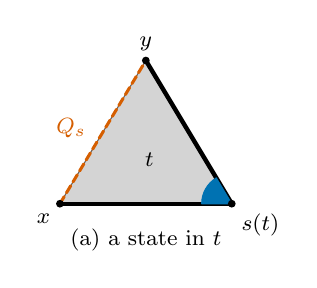
\begin{tikzpicture}[x=0.075\textwidth,y=0.075\textwidth,font=\footnotesize,line cap=round,line join=round]
\coordinate (x) at (0,0); \coordinate (s) at (2.4,0); \coordinate (y) at (1.2,2);
\fill[bfblack] (x)--(s)--(y)--cycle; \draw[black!62,line width=.4pt] (x)--(s)--(y)--cycle;
\draw[black,line width=1.6pt] (x)--(s); \draw[black,line width=1.6pt] (s)--(y);
\draw[bfR,line width=1.1pt,dash pattern=on 3pt off 1.6pt] (x)--(y);
\path[fill=bfS,draw=bfS] (s) -- ++(180:0.42) arc[start angle=180,end angle=121,radius=0.42] -- cycle;
\foreach \p in {x,s,y} \fill (\p) circle[radius=1.4pt];
\node[anchor=north east] at (x) {$x$}; \node[anchor=north west] at (s) {$s(t)$}; \node[anchor=south] at (y) {$y$};
\node at (1.25,0.62) {$t$}; \node[text=bfR,anchor=east] at (0.5,1.05) {$Q_s$};
\node at (1.2,-0.5) {(a) a state in $t$};
\end{tikzpicture}\hspace{0.08\textwidth}
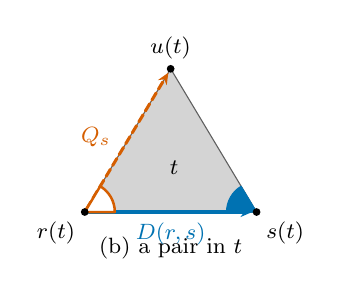
\begin{tikzpicture}[x=0.075\textwidth,y=0.075\textwidth,font=\footnotesize,line cap=round,line join=round]
\coordinate (r) at (0,0); \coordinate (s) at (2.4,0); \coordinate (u) at (1.2,2);
\fill[bfblack] (r)--(s)--(u)--cycle; \draw[black!62,line width=.4pt] (r)--(s)--(u)--cycle;
\draw[bfS,line width=1.1pt,shorten >=1.6pt,shorten <=1.2pt,-{Stealth[length=4.2pt,width=3.6pt]}] (r)--(s);
\draw[bfR,line width=1.1pt,dash pattern=on 3pt off 1.6pt,shorten >=1.6pt,shorten <=1.2pt,-{Stealth[length=4.2pt,width=3.6pt]}] (r)--(u);
\path[fill=bfS,draw=bfS] (s) -- ++(180:0.42) arc[start angle=180,end angle=121,radius=0.42] -- cycle;
\path[fill=white,draw=bfR,line width=.9pt] (r) -- ++(0:0.42) arc[start angle=0,end angle=59,radius=0.42] -- cycle;
\foreach \p in {r,s,u} \fill (\p) circle[radius=1.4pt];
\node[anchor=north east] at (r) {$r(t)$}; \node[anchor=north west] at (s) {$s(t)$}; \node[anchor=south] at (u) {$u(t)$};
\node at (1.25,0.62) {$t$}; \node[text=bfS,anchor=north] at (1.2,-0.02) {$D(r,s)$}; \node[text=bfR,anchor=east] at (0.5,1.05) {$Q_s$};
\node at (1.2,-0.5) {(b) a pair in $t$};
\end{tikzpicture}
\caption{One black triangle $t\in A$. (a) A state chooses the corner $s(t)$ (solid wedge). A selection built from $s$ uses one of the two bold sides at $s(t)$; the dashed side opposite $s(t)$ is the edge of $Q_s$ in $t$. (b) A pair (Section~\ref{sec:pairs}) adds a second corner $r(t)\neq s(t)$ (outlined wedge). The arrow $r(t)\to s(t)$ is the edge of $D(r,s)$ in $t$, and the partner directs the edge of $Q_s$ from $r(t)$ to the third corner $u(t)$.}
\label{fig:local}
\end{figure}

\begin{example}\label{ex:states}
In the example, $t_0=\{0,4,5\}$, $e_0=\{0,4\}$, $c=5$ and $n=10$.
Two of its states, which we call $\alpha$ and $\beta$, are
\[
\begin{array}{c|cccccccccc}
t & 016 & 023 & 178 & 129 & 349 & 4\,10\,11 & 5\,6\,11 & 6\,7\,12 & 8\,11\,12 & 8\,9\,10\\\hline
\alpha(t) & 1 & 3 & 7 & 2 & 9 & 11 & 6 & 12 & 8 & 10\\
\beta(t) & 6 & 2 & 8 & 1 & 3 & 10 & 11 & 7 & 12 & 9
\end{array}
\]
where a face is named by its corners.
The sides opposite $\alpha$ contain the triangle on $1,8,9$, while those opposite $\beta$ form a forest with components $\{0,1,3,7\}$, $\{2,4,8,9,10,11\}$ and $\{5,6,12\}$, one root in each (Figure~\ref{fig:Q}).
The two states differ in every face; we come back to this in Section~\ref{sec:pairs}.
\end{example}

\begin{figure}[tb]
\centering
\includegraphics[width=0.94\textwidth]{\FIG 09-Q.pdf}
\caption{The opposite sides (dashed) of the two states of Example~\ref{ex:states}; solid wedges mark the chosen corners and hollow circles the roots. (a) $Q_\alpha$ contains the triangle on $1,8,9$ around a white face, and its component has no root. (b) $Q_\beta$ is a forest with three components, one through each root. The proof needs a state that looks like (b).}
\label{fig:Q}
\end{figure}

\subsection*{The tree of faces}
A selection that contains $e_0$ and uses only sides at $s(t)$ in each $t\in A$ is a selection that avoids $S_s$.
It pairs each face with the face across its selected side, and these two faces are adjacent across an edge not in $S_s$.
So consider the graph $Y_s=\T^*-S_s^*$, whose nodes are the faces of $\T$, two faces being adjacent when they share a side not in $S_s$; it is a subgraph of $G$.
For this graph to be a tree we need the following condition on $s$.

\begin{definition}
A state $s$ is \emph{good} if $Q_s$ is a forest in which each component contains exactly one root.
\end{definition}

\begin{lemma}\label{lem:good}
A state $s$ is good if and only if $S_s$ is a spanning tree of $\T$.
\end{lemma}

\begin{proof}
$S_s$ has $|V(\T)|-1$ edges, so it is a spanning tree exactly when it is acyclic.
That happens exactly when $Q_s$ is acyclic and adding $ac$ and $bc$ closes no cycle, that is, when $a$, $b$ and $c$ lie in three different components of $Q_s$.
A forest with $n$ edges on $n+3$ vertices has three components, so this means one root in each.
\end{proof}

\begin{lemma}\label{lem:Y}
Let $s$ be a good state.
Then $Y_s$ is a tree on the $2k$ faces of $\T$, in which every face of $A$ has degree two and $t_0$ has degree one.
Root $Y_s$ at $t_0$, and let $P_s$ consist of the side that each black face shares with its child.
Then $P_s$ is a selection, $e_0\in P_s$, and for every $t\in A$ the side of $t$ in $P_s$ contains $s(t)$.
\end{lemma}

\begin{proof}
$Y_s$ is a spanning tree of $G$ by Lemmas~\ref{lem:good} and~\ref{lem:duality}(2).
A face $t\in A$ has exactly one side in $S_s$, its side in $Q_s$, because $ac$ and $bc$ belong to $t_0$; so $t$ has degree two.
The face $t_0$ has $ac,bc\in S_s$ and $e_0\notin S_s$, so it has degree one, and its neighbour is the white face $y_0$ across $e_0$.
Colours alternate along every edge of $Y_s$.
In the rooted tree, $t_0$ has one child, every $t\in A$ has a parent and so exactly one child, and every white face has a parent, which is black.
Thus every black face has exactly one side in $P_s$.
A white face $y$ is the only child of its parent, so the side towards its parent is in $P_s$.
Any other side of $y$ would be shared with a black child $t$ of $y$, and the side that $t$ selects is shared with the child of $t$, which is not $y$; since two faces share at most one side, that side is not in $P_s$.
So every white face has exactly one side in $P_s$.
The side that $t_0$ shares with $y_0$ is $e_0$, and for $t\in A$ the side shared with its child is not in $Q_s$, so it is one of the two sides at $s(t)$.
\end{proof}

For a good state Lemma~\ref{lem:Y} produces a selection $P_s$ containing $e_0$ without any further choice.
It remains to see that $P_s$ has no cycle.
A cycle in $P_s\setminus\{e_0\}$ would be made of sides leaving chosen corners, and the rest of this section says what such a cycle looks like.

\subsection*{The inside of a cycle}
Throughout the paper, the cycles we need are made of sides leaving corners chosen by a state.
Let $r$ be a state (we will apply this to both states of a pair, which is why it is called $r$), and suppose that in every face $t\in A$ one of the two sides at $r(t)$ has been chosen and directed out of $r(t)$.
We call these the \emph{chosen sides}.
One principle about them is used four times.

\begin{lemma}[outdegree]\label{lem:outdegree}
Let $F$ be a set of edges of $\T$, each directed, such that every vertex has at most one outgoing edge in $F$.
Then every cycle of $F$ is a directed cycle.
A component of $F$ with $q$ vertices, of which $\gamma$ have no outgoing edge, has $q-\gamma$ edges; so $\gamma\le1$, the component is a tree if $\gamma=1$, and it contains exactly one cycle if $\gamma=0$.
\end{lemma}

\begin{proof}
A cycle with $h$ edges has $h$ distinct tails on its $h$ vertices, so every vertex is the tail of one of its edges.
The edge count is the sum of the outdegrees, and a connected graph with $q$ vertices has at least $q-1$ edges, with equality for a tree, and exactly one cycle if it has $q$.
\end{proof}

The chosen sides have outdegree one at every vertex of $X$ and zero at the roots, so Lemma~\ref{lem:outdegree} applies.
Let $Z$ be a directed cycle of chosen sides, of length $h$.
Every vertex of $Z$ has an outgoing chosen side, so it lies in $X$.
The roots lie on the boundary of the outer face, and not on $Z$, so they lie outside $Z$; hence every black face inside $Z$ lies in $A$.
Let $B$ and $W$ be the numbers of black and white faces inside $Z$, let $I$ be the number of vertices strictly inside, and let $\ell$ be the number of edges of $Z$ whose black face is inside.

Euler's formula needs a connected plane graph, so we first say what the inside of $Z$ is.
Let $R_Z$ consist of $Z$ and the vertices and edges of $\T$ inside $Z$.
By the Jordan curve theorem the outside of $Z$ is an open disk; it contains no point of $R_Z$ and its boundary is $Z$, so it is one face of $R_Z$, bounded by the cycle $Z$.
Every other face of $R_Z$ lies inside $Z$ and contains no vertex or edge of $\T$, so it lies in one face of $\T$; conversely a face of $\T$ inside $Z$ is a connected region disjoint from $R_Z$ whose boundary triangle lies in $R_Z$.
So the faces of $R_Z$ are the $B+W$ faces of $\T$ inside $Z$ and the outside of $Z$, each bounded by a cycle, and $R_Z$ is connected by Lemma~\ref{lem:connected}.
A vertex strictly inside $Z$ has all its faces inside $Z$, so no vertex is pinched between the two sides.

\begin{lemma}[disk identity]\label{lem:disk}
In this situation $W=B+1$ and $h=2\ell+3$.
In particular $h$ is odd and $Z$ encloses at least one white face.
\end{lemma}

\begin{proof}
Two counts hold for every cycle of $\T$.
The plane graph $R_Z$ has $I+h$ vertices, $B+W+1$ faces, and $(3(B+W)+h)/2$ edges, since each inner face has three sides, an edge strictly inside lies on two inner faces and an edge of $Z$ on one; Euler's formula gives the first count below.
For the second, count each side of an inner face with $+1$ if the face is black and $-1$ if it is white: an edge strictly inside contributes $+1-1$, and an edge of $Z$ contributes $+1$ or $-1$ according to its inner face.
Thus
\[
B+W=2I+h-2,\qquad 3(B-W)=2\ell-h .
\]
The third count uses the state.
Send each black face $t$ inside $Z$ to $r(t)$, a vertex inside or on $Z$.
This is injective because $r$ is.
Every vertex $v$ strictly inside is hit: $v=r(t)$ for some $t\in A$ because $r$ is onto $X$, and $t$ has the corner $v$, so it lies inside.
A vertex $v$ on $Z$ is $r(t)$ for exactly one $t$, and the edge of $Z$ leaving $v$ is the chosen side of that $t$, because each face has only one chosen side and $r$ is injective; so $v$ is hit exactly when that edge has its black face inside.
This happens for $\ell$ vertices of $Z$, so
\[
B=I+\ell .
\]
Substituting into the first count gives $W=I+h-\ell-2$, hence $B-W=2\ell-h+2$, and the second count becomes $3(2\ell-h+2)=2\ell-h$, that is $h=2\ell+3$; then $W-B=h-2\ell-2=1$.
\end{proof}

Only the third count uses the state, and it uses both halves of bijectivity: injectivity so that no vertex is counted twice, surjectivity so that every interior vertex is counted.
Without it the conclusion fails for cycles of $\T$ in general.
Figure~\ref{fig:disk} shows the five numbers on a cycle of the example.

\begin{figure}[tb]
\centering
\includegraphics[width=0.78\textwidth]{\FIG 08-disk.pdf}
\caption{The disk identity on the $7$-cycle $1,2,3,9,10,11,6$, whose arrows leave the corners chosen by the state $\beta$ of Example~\ref{ex:states} (outlined wedges); it is the long cycle of Figure~\ref{fig:pair}. The tinted disk has $B=5$ black and $W=6$ white faces, $I=3$ vertices strictly inside (ringed: $7,8,12$) and $h=7$ edges, of which $\ell=2$ have their black face inside (marked). Each black face inside holds one outlined wedge, at a ringed vertex or at the tail of a marked arrow, which is the count $B=I+\ell$. So $W=B+1$ and $h=2\ell+3$, equivalently $2\ell-h=-3$.}
\label{fig:disk}
\end{figure}

\subsection*{The recovered selection has no cycle}

\begin{proposition}\label{prop:recover}
If $s$ is a good state, then $P_s$ is an acyclic selection containing $e_0$.
Consequently, if $\T$ has a good state for $t_0$ and $e_0$, then $G$ has a Hamiltonian cycle avoiding the edge that crosses $e_0$.
\end{proposition}

\begin{proof}
By Lemma~\ref{lem:Y}, $P_s$ is a selection containing $e_0$.
Let $P_0=P_s\setminus\{e_0\}$ and direct the side of each $t\in A$ in $P_0$ out of $s(t)$, which is one of its ends.
These are chosen sides for the state $s$.

Suppose $P_0$ contains a cycle $Z$.
By Lemma~\ref{lem:outdegree} it is a directed cycle of chosen sides, so the disk identity gives $W-B=1$ and $h-2\ell=3$.
Now count the faces inside $Z$ through $P_s$, which matches every face with the face across its selected side.
The selected side of a face inside $Z$ lies in the closed disk; it is not $e_0$, whose ends are roots.
If it is strictly inside $Z$, it matches the face with another face inside $Z$ of the other colour.
Every edge of $Z$ lies in $P_s$, so it is the selected side of both its faces, one inside and one outside.
Thus exactly $\ell$ black faces and $h-\ell$ white faces inside $Z$ are matched across $Z$, and the others are matched in pairs inside.
Hence $B-\ell=W-(h-\ell)$, that is $W-B=h-2\ell=3$, contradicting $W-B=1$.

So $P_0$ is a forest, and by Lemma~\ref{lem:outdegree} each component contains exactly one root.
The edge $e_0=ab$ joins the components of $a$ and $b$, so $P_s=P_0\cup\{e_0\}$ is acyclic.
The last sentence follows from Proposition~\ref{prop:target}(1).
\end{proof}

In words: a cycle of chosen sides encloses one more white face than black, but a selection running along it would force three more.

\begin{example}\label{ex:recover}
The state $\beta$ of Example~\ref{ex:states} is good.
Its selection $P_\beta$ has eleven edges forming two trees, on $\{0,2,4,6,7,8\}$ and $\{1,3,5,9,10,11,12\}$, and Figure~\ref{fig:selected} shows it with the Hamiltonian cycle of $G$ that crosses the other $22$ edges.
The example has six good states, and they give six different Hamiltonian cycles avoiding the edge of $G$ that crosses $e_0$; these are all such cycles of this $G$.
On the cube (Figure~\ref{fig:cube}), with $t_0=\{0,1,2\}$ and $e_0=\{0,1\}$, both states are good; for $s$ the tree $Y_s$ makes the black faces $135$, $234$, $045$ select $35$, $23$, $04$, and with $e_0$ these form the trees on $\{0,1,4\}$ and $\{2,3,5\}$.
\end{example}

\begin{figure}[tb]
\centering
\includegraphics[width=0.94\textwidth]{\FIG 13-selected.pdf}
\caption{The selection $P_\beta$ (bold). (a) The dash-dotted tree is $Y_\beta$ with its black nodes suppressed: a tree on the white faces rooted at the ringed face $y_0$ across $e_0=\{0,4\}$. The root selects $e_0$, and every other white face selects the side towards its parent. Every face has one bold side. (b) The bold edges form two trees, on the disks and on the squares, and the curve that crosses each other edge once is the Hamiltonian cycle of $G$ through all $22$ faces.}
\label{fig:selected}
\end{figure}

So Theorem~\ref{thm:main} follows once we find a good state, and once we can deal with triangulations that have none.
Section~\ref{sec:pairs} finds a good state from a pair of states, Section~\ref{sec:flow} finds a pair when $\T$ has no separating triangle, and Section~\ref{sec:glue} removes separating triangles.

\FloatBarrier
\section{Pairs of states}\label{sec:pairs}

\subsection*{Why a second state}
Goodness asks two things of $Q_s$: no cycle, and one root per component.
The second condition concerns whole components.
A second state $r$ that differs from $s$ in every face turns it into the first: it gives every vertex of $X$ exactly one outgoing edge of $Q_s$, and then a component without a cycle contains exactly one root.

\begin{definition}
A \emph{pair} is an ordered pair $(r,s)$ of states with $r(t)\neq s(t)$ for every $t\in A$; we call $r$ a \emph{partner} of $s$, and $s$ the \emph{second state}.
For a pair we write $u(t)$ for the third corner of $t$.
\end{definition}

\begin{lemma}\label{lem:partner}
Let $(r,s)$ be a pair, and direct the edge of $Q_s$ in each $t\in A$ from $r(t)$ to $u(t)$.
Then every vertex of $X$ has outdegree one and every root outdegree zero.
Each component of $Q_s$ either is a tree containing exactly one root, or contains no root and exactly one cycle, which is directed.
So $s$ is good if and only if $Q_s$ is acyclic, and a good state has exactly one partner.
\end{lemma}

\begin{proof}
The edge of $Q_s$ in $t$ joins $r(t)$ and $u(t)$, and $r$ is a bijection onto $X$, which gives the outdegrees; the rest of the first two sentences is Lemma~\ref{lem:outdegree}.
If $s$ is good, a partner must direct each tree of $Q_s$ towards its root, and $r(t)$ is the tail of the edge of $Q_s$ in $t$; so $r$ is determined.
Conversely, directing the trees towards their roots and taking tails defines a bijection $r\colon A\to X$ with $r(t)\neq s(t)$, because the edge of $Q_s$ in $t$ avoids $s(t)$.
\end{proof}

Besides $Q_s$ a pair gives the set $D(r,s)$ of edges $r(t)\to s(t)$, $t\in A$ (Figure~\ref{fig:local}(b)).
Every vertex of $X$ is $r(t)$ for one $t$ and $s(t')$ for one $t'$, so it has one outgoing and one incoming edge in $D(r,s)$.
The edges come from distinct black faces, so they are distinct even as undirected edges, and $\T$ is simple.
Hence $D(r,s)$ is a union of disjoint directed cycles of $\T$, each of length at least three, covering $X$, and each face $t\in A$ supplies one edge to exactly one of them.
The edges of $D(r,s)$ are chosen sides for the state $r$, and so are the edges of $Q_s$ directed as in Lemma~\ref{lem:partner}.
So the disk identity applies to every cycle of $D(r,s)$ and to every cycle of $Q_s$.

\begin{figure}[tb]
\centering
\includegraphics[width=0.94\textwidth]{\FIG 07-pair-D.pdf}
\caption{The pair $(\beta,\alpha)$ of Example~\ref{ex:states}: outlined wedges mark $\beta$, solid wedges $\alpha$. (b) The arrows $\beta(t)\to\alpha(t)$ form $D(\beta,\alpha)$, a counterclockwise cycle of length $7$ through $6,1,2,3,9,10,11$ and a clockwise triangle through $8,7,12$.}
\label{fig:pair}
\end{figure}

In the example $(\beta,\alpha)$ is a pair (Figure~\ref{fig:pair}), and so is $(\alpha,\beta)$.
The second state of $(\alpha,\beta)$ is good, and the second state of $(\beta,\alpha)$ is not.

\subsection*{Two reversals}
A pair can be changed along a cycle in two ways, which Table~\ref{tab:reversals} sets side by side.

\begin{lemma}\label{lem:reversals}
Let $(r,s)$ be a pair.
\begin{enumerate}
\item Let $K$ be a cycle of $Q_s$, and put $\tilde r(t)=u(t)$ for the faces $t$ whose edge lies on $K$ and $\tilde r(t)=r(t)$ otherwise.
Then $(\tilde r,s)$ is a pair, $\tilde r$ directs $K$ the other way round, and the same operation applied to $(\tilde r,s)$ and $K$ returns $(r,s)$.
\item Let $C$ be a cycle of $D(r,s)$, and exchange $r(t)$ and $s(t)$ for the faces $t$ whose edge lies on $C$.
The result is a pair whose set of $D$-edges is $D(r,s)$ with $C$ reversed.
\end{enumerate}
\end{lemma}

\begin{proof}
(1) By Lemma~\ref{lem:partner} the cycle $K$ is directed by $r$, so $r$ maps its faces onto the tails of its edges, which are all its vertices, and $u$ maps them onto the heads, again all its vertices.
So $\tilde r$ is a bijection, and $\tilde r(t)=u(t)\neq s(t)$.
On the faces of $K$ the corners $r(t)$ and $u(t)$ trade roles, so $K$ is reversed and the operation undoes itself.
(2) The tails and the heads of $C$ are both its vertex set, so both new maps are bijections, and they still differ on every face.
\end{proof}

\begin{table}[tb]
\centering
\begin{tabular}{@{}lllll@{}}
\toprule
reversal of & changes & keeps & sign & used for\\
\midrule
a cycle of $Q_s$ & $r$ on its faces & $s$, so $Q_s$ and $F(s)$ & flips & cancelling cyclic $Q_s$\\
a cycle of $D(r,s)$ & $r$ and $s$ on its faces & undirected $D$ & flips & showing the sum is not $0$\\
\bottomrule
\end{tabular}
\vspace{4pt}
\caption{The two reversals of Lemma~\ref{lem:reversals}. The sign is that of Lemma~\ref{lem:sign}.}
\label{tab:reversals}
\end{table}

\subsection*{A sign}
We want to count pairs so that the pairs with cyclic $Q_s$ cancel.
Reversing a cycle of $Q_s$ pairs them up, so we need a sign that this reversal changes.
For adjacent vertices $v,w$ put $\delta(v,w)=1$ if the black face of the edge $vw$ lies to the left of $v\to w$, and $\delta(v,w)=-1$ otherwise; equivalently $\delta(v,w)=1$ when $w$ follows $v$ in the counterclockwise order of the corners of that black face.
Along a directed cycle $Z$ of $\T$ traversed counterclockwise the inside is on the left, so the sum of $\delta$ along $Z$ is $\ell-(h-\ell)=2\ell-h$, and by the disk identity a counterclockwise cycle of chosen sides has $\delta$-sum $-3$ and a clockwise one $+3$.
For a pair put
\[
\eps(r,s)=\prod_{t\in A}\delta\bigl(r(t),s(t)\bigr).
\]

\begin{lemma}\label{lem:sign}
Both reversals of Lemma~\ref{lem:reversals} change the sign $\eps$.
If $D(r,s)$ has $c$ cycles, of which $c^+$ run counterclockwise, then $n\equiv c\pmod 2$ and
\[
\eps(r,s)=(-1)^{(n+c)/2}(-1)^{c^+}.
\]
\end{lemma}

\begin{proof}
In a black triangle with corners $r,s,u$ the three directed edges $r\to s$, $s\to u$, $u\to r$ run the same way round the triangle, so they have the same $\delta$, and $\delta(u,s)=-\delta(s,u)=-\delta(r,s)$.
Reversing a cycle $K$ of $Q_s$ replaces $\delta(r(t),s(t))$ by $\delta(u(t),s(t))$ on the faces of $K$; reversing a cycle $C$ of $D(r,s)$ replaces it by $\delta(s(t),r(t))$.
In both cases every factor on the cycle changes sign, and the cycle has odd length by the disk identity, so $\eps$ changes sign.

A cycle of $D(r,s)$ of length $h$ has $h$ factors $\pm1$ with sum $-3$ if it runs counterclockwise and $+3$ if clockwise, so it has $(h+3)/2$ or $(h-3)/2$ factors $-1$.
The lengths are odd and add up to $|X|=n$, so $c\equiv n$, and the total number of factors $-1$ is $(n-3c)/2+3c^+$, which has the parity of $(n+c)/2+c^+$.
\end{proof}

The reversal of a cycle of $Q_s$ can rearrange the cycles of $D$ completely, so a sign defined by counting the cycles of $D$ would not be controlled.
The product of local signs changes in a computable way under both reversals, and the disk identity makes the number of changed factors odd.

\subsection*{Cancellation}

\begin{lemma}\label{lem:cancel}
Let $s$ be a state for which $Q_s$ contains a cycle.
Then $\sum_r\eps(r,s)=0$, the sum running over the partners $r$ of $s$.
Consequently, for every function $F$ on states,
\[
\sum_{(r,s)\ \text{pair}}\eps(r,s)\,F(s)=\sum_{s\ \text{good}}F(s)\,\eps(r_s,s),
\]
where $r_s$ is the partner of the good state $s$.
\end{lemma}

\begin{proof}
Fix an order on the cycles of $\T$, and let $K_s$ be the first cycle of $Q_s$; it depends on $s$ only.
For a partner $r$ of $s$, reverse $K_s$ as in Lemma~\ref{lem:reversals}(1).
The new partner $\tilde r$ has the same second state $s$, hence the same $Q_s$ and the same $K_s$, and reversing again gives back $r$.
This is an involution on the partners of $s$ without fixed points, and by Lemma~\ref{lem:sign} it changes $\eps$, so the sum is zero.
For the second statement group the pairs by $s$: the states with a partner and acyclic $Q_s$ are the good states, each with one partner, by Lemma~\ref{lem:partner}.
\end{proof}

The cycle $K_s$ must be chosen from $s$ alone; a rule that looked at $r$ might pick a different cycle after the reversal, and the map would not be an involution.
In the example only $\alpha$ has a cycle in $Q_\alpha$, and its two partners are $\beta$ and the state $\tilde\beta$ obtained by reversing the triangle $8,1,9$, which changes $\beta$ in the faces $178$, $129$, $89\,10$ from $8,1,9$ to $1,9,8$ (Figure~\ref{fig:cancel}).

\begin{figure}[tb]
\centering
\includegraphics[width=0.94\textwidth]{\FIG 10-cancellation.pdf}
\caption{Cancellation in the example ($n=10$). (a) The pair $(\beta,\alpha)$. Dashed edges are $Q_\alpha$; its cycle $1,8,9$ (heavy, around the tinted white face) is directed by $\beta$ from the outlined corner to the third corner. (b) Reversing that cycle moves the outlined wedges in its three faces to their third corners and leaves the solid wedges, the state $\alpha$, unchanged. Three local signs flip, so $\eps$ changes sign and the two pairs cancel in any sum weighted by a function of the second state.}
\label{fig:cancel}
\end{figure}

\subsection*{Heights}
Lemma~\ref{lem:cancel} turns the search for a good state into a question: is there a function $F$ of the second state for which $\sum_{(r,s)}\eps(r,s)F(s)\neq0$?
With $F=1$ the answer is no, since reversing the cycle of $D(r,s)$ through a fixed vertex pairs every pair with one of opposite sign.
So $F$ must tell apart the two orientations of a cycle of $D$.
The disk identity offers a way, because every such cycle encloses a white face.
For each white face we walk from it to the outer face and record, at every black face on the way, whether the walk passes the chosen corner.

For each white face $y$ fix a path of faces $y=f_0,f_1,\dots,f_j=t_0$ in $G$: consecutive faces share a side, and no face is repeated.
Such a path exists because $G$ is connected.
A black face $t\in A$ on the path is entered across one of its sides and left across another.
These two sides meet in one corner $v$ of $t$, and we say that the path \emph{turns around} $v$ in $t$.
Put $\kappa_y(t,v)=1$ if the path turns around $v$ in $t$ with $v$ on its left, $\kappa_y(t,v)=-1$ if it turns around $v$ with $v$ on its right, and $\kappa_y(t,v)=0$ if the path misses $t$ or turns around another corner of $t$.
(Combinatorially: if $a'$ is the far end of the side of entry and $b'$ the far end of the side of exit, then $v$ is on the left exactly when $v,a',b'$ is the counterclockwise order of the corners of $t$.)
The \emph{height} of a state $s$ at $y$ and its \emph{weight} are
\[
\eta_s(y)=\sum_{t\in A}\kappa_y\bigl(t,s(t)\bigr),\qquad \omega(s)=\sum_{y\ \text{white}}\eta_s(y).
\]
The paths are fixed once and for all; Figure~\ref{fig:heights} shows one.

\begin{figure}[tb]
\centering
\includegraphics[width=0.94\textwidth]{\FIG 17-heights.pdf}
\caption{A height in the example. The white face $y=\{1,8,9\}$ (tinted) and its path of faces to the outer face (dash-dotted): $y$, $\{1,7,8\}$, $\{1,6,7\}$, $\{0,1,6\}$, $\{0,5,6\}$, $t_0$. In each black face on the path the path turns around one corner; the circled sign is $+$ if that corner lies on its left and $-$ if on its right. The height of a state at $y$ adds the signs at turned corners that carry its wedge. (a) The pair obtained from $(\beta,\alpha)$ by reversing the $7$-cycle, which now runs clockwise. Its second state $s$ has its wedge at the turned corner $6$ of $\{0,1,6\}$ and not at the turned corner $1$ of $\{1,7,8\}$, so $\eta_s(y)=-1$. (b) The pair $(\beta,\alpha)$, with the $7$-cycle counterclockwise. The wedge in $\{0,1,6\}$ has moved to $1$, and $\eta_\alpha(y)=0$, one more, because $y$ lies inside the $7$-cycle.}
\label{fig:heights}
\end{figure}

\begin{lemma}\label{lem:height}
Let $(r,s)$ be a pair, $C$ a clockwise cycle of $D(r,s)$, and $(r',s')$ the pair obtained by reversing $C$.
Then $\eta_{s'}(y)-\eta_s(y)$ is $1$ if the white face $y$ lies inside $C$ and $0$ otherwise.
Hence $\omega(s')-\omega(s)=L(C)$, the number of white faces inside $C$, and $L(C)\ge1$.
\end{lemma}

\begin{proof}
After the reversal $C$ runs counterclockwise, with edges $s(t)\to r(t)$, and $s'(t)=r(t)$ on its faces.
So $\eta_{s'}(y)-\eta_s(y)=\sum_t\bigl(\kappa_y(t,r(t))-\kappa_y(t,s(t))\bigr)$ over the faces $t$ whose edge lies on $C$.
Fix such a face $t$ and let $g$ be its side on $C$, which joins $s(t)$ and $r(t)$.
If the path of $y$ misses $t$ or turns around $u(t)$ in $t$, it does not cross $g$ on its way through $t$, and the summand of $t$ is $0$.
Otherwise it crosses $g$ once on its way through $t$.
We claim that the summand is then $+1$ if this crossing leads from the left of $s(t)\to r(t)$ to its right, and $-1$ if it leads from right to left.
Suppose it leads from left to right.
If $t$ lies on the left of $s(t)\to r(t)$, the path leaves $t$ across $g$, and the corners of $t$ in counterclockwise order are $s(t),r(t),u(t)$.
Either the path entered across $r(t)u(t)$ and turns around $r(t)$, which is then on its left, or it entered across $s(t)u(t)$ and turns around $s(t)$, which is then on its right.
In both cases the summand is $+1$.
If $t$ lies on the right of $s(t)\to r(t)$, the path enters $t$ across $g$, and the same check gives $+1$.
Reversing the direction of travel exchanges left and right, which gives $-1$ for a crossing from right to left.

Every step of the path across an edge of $C$ enters or leaves the black face of that edge, which lies in $A$ and so is not an end of the path; and the path passes through that face only once.
So the sum over $t$ is the number of steps that cross $C$ from left to right minus the number that cross from right to left.
The left of the counterclockwise cycle $C$ is its inside, and by Lemma~\ref{lem:duality}(1) a step changes sides of $C$ exactly when it crosses an edge of $C$.
The path ends in $t_0$, which is outside $C$, so the sum is $1$ if $y$ is inside $C$ and $0$ otherwise.
Finally $L(C)\ge1$ by the disk identity.
\end{proof}

Since $\eta_s(y)$ is a sum over faces, and different cycles of $D(r,s)$ use different faces, the effects of reversing several cycles add up.
These heights are the weights that OpenAI construct in the proof of \cite[Lemma~5.3]{openai2026} for one choice of their circulations, read face by face, and they are the half-ray counts of Li \cite[Section~4]{li2026} taken along fixed paths.

\subsection*{The total is not zero}
Let $m\ge1$ be the smallest number of cycles of $D(r,s)$ over all pairs, assuming a pair exists, and take $F=\omega^m$.
Here is why a power.
Pairs with the same undirected edges of $D$ differ only in the orientations of the cycles, and by Lemma~\ref{lem:height} the weight $\omega$ is a constant plus one term for each cycle that runs counterclockwise.
The sign alternates with each orientation, so the signed sum over such pairs is a repeated difference, one for each cycle.
A difference taken $c$ times kills every polynomial of degree less than $c$, and on a polynomial of degree $c$ it leaves only the product of the $c$ steps.

\begin{lemma}\label{lem:difference}
Let $\omega_0,L_1,\dots,L_c$ be real numbers and $m\le c$ a nonnegative integer.
Then
\[
\sum_{x\in\{0,1\}^c}(-1)^{x_1+\dots+x_c}\bigl(\omega_0+x_1L_1+\dots+x_cL_c\bigr)^m
=\begin{cases}0 & \text{if } m<c,\\ (-1)^c\,c!\,L_1\cdots L_c & \text{if } m=c.\end{cases}
\]
\end{lemma}

\begin{proof}
Expand the power and use $x_i^j=x_i$ for $x_i\in\{0,1\}$ and $j\ge1$.
Every term becomes a constant times $\prod_{i\in I}x_i$ for a set $I$ with $|I|\le m$.
For such a product the sum over $x$ factors into one sum for each $i$: $\sum_{x_i}(-1)^{x_i}x_i=-1$ if $i\in I$ and $\sum_{x_i}(-1)^{x_i}=0$ if $i\notin I$.
So it vanishes unless $I=\{1,\dots,c\}$, which needs $m=c$; those terms arise by taking a different $x_iL_i$ from each of the $c$ factors, in $c!$ ways.
\end{proof}

\begin{proposition}\label{prop:good}
If $\T$ has a pair, then it has a good state.
\end{proposition}

\begin{proof}
Let $\Sigma=\sum_{(r,s)}\eps(r,s)\,\omega(s)^m$ over all pairs.
By Lemma~\ref{lem:cancel} it is a sum over good states, so it suffices to show $\Sigma\neq0$.

Sort the pairs into classes by the undirected edge set of $D(r,s)$.
Fix a pair $(r,s)$ whose $D$ has cycles $C_1,\dots,C_c$, and a pair $(r',s')$ with the same undirected edges.
This edge set contains exactly one side of each face $t\in A$, so $(r'(t),s'(t))=(r(t),s(t))$ or $(s(t),r(t))$.
Along a cycle consecutive faces make the same choice, since if exactly one of the two edges at a vertex $x$ were reversed, $x$ would be the value of $r'$, or of $s'$, at two faces.
So the class of $(r,s)$ consists of the $2^c$ pairs obtained by reversing some of its cycles, which are pairs by Lemma~\ref{lem:reversals}(2).
Index them by $x\in\{0,1\}^c$, with $x_i=1$ when $C_i$ runs counterclockwise.
By Lemma~\ref{lem:sign}, $\eps=(-1)^{(n+c)/2}(-1)^{x_1+\dots+x_c}$, and by Lemma~\ref{lem:height}, $\omega=\omega_0+x_1L(C_1)+\dots+x_cL(C_c)$, where $\omega_0$ is the weight of the second state when every cycle runs clockwise.
Every class has $c\ge m$, so by Lemma~\ref{lem:difference} the class contributes $0$ if $c>m$, and
\[
(-1)^{(n+m)/2}(-1)^m\,m!\,L(C_1)\cdots L(C_m)=(-1)^{(n-m)/2}\,m!\,L(C_1)\cdots L(C_m)
\]
if $c=m$.
At least one class has $c=m$, and every $L(C_i)\ge1$, so
\[
\Sigma=(-1)^{(n-m)/2}\,m!\sum\ \prod_{i=1}^m L(C_i)\neq0,
\]
the sum running over the classes with $m$ cycles.
\end{proof}

The minimum cannot be dropped: a class with $c$ cycles contributes with the sign $(-1)^{(n-c)/2}$ in its leading term, and this sign alternates as $c$ grows by two.
Only the classes with the fewest cycles are sure to agree.

\begin{example}\label{ex:count}
In the example the $8$ pairs fall into two classes of four, both with $m=2$ cycles: a $7$-cycle enclosing $6$ white faces and a triangle enclosing $1$ (the class of $(\beta,\alpha)$), and a $7$-cycle enclosing $3$ and a triangle enclosing $1$.
Table~\ref{tab:pairs} lists all eight, with the weights of the paths of faces chosen as shortest paths.
In each class the four values of $\eps\,\omega^2$ add up to $2\,L_1L_2$: $16-9-4+9=12$ and $4-1-1+4=6$.
So $\Sigma=18$, while $\sum\eps=\sum\eps\,\omega=0$.
The two pairs with a cycle in $Q_s$ have the same second state $\alpha$ and cancel; the six good states are the second states of the other six pairs, three with $\eps=+1$ and three with $\eps=-1$.
\end{example}

\begin{table}[tb]
\centering
\begin{tabular}{@{}cccrrl@{}}
\toprule
class & $7$-cycle & triangle & $\eps$ & $\omega(s)$ & second state $s$ \\
\midrule
$L=6,1$ & cw & cw & $+1$ & $-4$ & good \\
$L=6,1$ & cw & ccw & $-1$ & $-3$ & good ($s=\beta$) \\
$L=6,1$ & ccw & cw & $-1$ & $2$ & cycle in $Q_s$ ($s=\alpha$) \\
$L=6,1$ & ccw & ccw & $+1$ & $3$ & good \\
\midrule
$L=3,1$ & cw & cw & $+1$ & $-2$ & good \\
$L=3,1$ & cw & ccw & $-1$ & $-1$ & good \\
$L=3,1$ & ccw & cw & $-1$ & $1$ & good \\
$L=3,1$ & ccw & ccw & $+1$ & $2$ & cycle in $Q_s$ ($s=\alpha$) \\
\bottomrule
\end{tabular}
\vspace{4pt}
\caption{The eight pairs of the example. Reversing the $7$-cycle from clockwise to counterclockwise raises $\omega$ by $L=6$ or $3$, reversing the triangle raises it by $1$, and each reversal flips $\eps$.}
\label{tab:pairs}
\end{table}

\begin{remark}\label{rem:other-sums}
OpenAI test the signed count against $\exp(x\,\omega(s))$ with the phase $i^{J}$, where $J=\frac13\sum_t\delta(r(t),s(t))$, and read off the Taylor coefficient of order $m$.
Since $i^{J}=i^{-n}\eps$, that coefficient is $i^{-n}\Sigma/m!$.
The unsigned manuscript \cite{constructive2026} uses the integer polynomial $\sum\eps(r,s)z^{\omega(s)}$ and its coefficient of $(z-1)^m$, which is $\sum\eps(r,s)\binom{\omega(s)}{m}=\Sigma/m!$, because the sums of $\eps\,\omega^j$ with $j<m$ vanish by Lemma~\ref{lem:difference}.
Li \cite{li2026} marks $m$ distinct crossings, which gives a symmetric function of degree $m$ in the crossing signs in place of the power.
None of these arguments is constructive.
\end{remark}

\FloatBarrier
\section{The first pair}\label{sec:flow}

Proposition~\ref{prop:good} needs one pair.
Let $\mathcal{B}$ be the bipartite graph on $A\cup X$ in which $t$ is joined to its corners in $X$.
States are the perfect matchings of $\mathcal{B}$.
A spanning subgraph of $\mathcal{B}$ with all degrees two is a union of disjoint even cycles, and taking alternate edges along each cycle splits it into two states that differ in every face, that is, a pair.
We find such a subgraph as a flow (Figure~\ref{fig:flow}).
Give the edges of a network capacity $2$ from a source to each $x\in X$, capacity $1$ from $x$ to each face $t\in A$ with corner $x$, and capacity $2$ from each $t\in A$ to a sink.
An integral flow of value $2n$ saturates every source and sink edge, and the incidences that carry flow form the required subgraph.
A cut with $S\subseteq X$ on the source side and the best placement of each $t$ has capacity $2(n-|S|)+\sum_{t\in A}\min\bigl(2,|V(t)\cap S|\bigr)$, where $V(t)$ is the set of corners of $t$.
By the integral max-flow min-cut theorem \cite{fordfulkerson1956}, a pair exists if
\begin{equation}\label{eq:hall}
\sum_{t\in A}\min\bigl(2,|V(t)\cap S|\bigr)\ \ge\ 2|S|\qquad\text{for all } S\subseteq X .
\end{equation}

\begin{figure}[tb]
\centering
\includegraphics[width=0.70\textwidth]{\FIG 06-flow.pdf}
\caption{The flow network for the example. Each vertex of $X$ receives at most $2$ from the source, each incidence (thin) carries at most $1$, and each black triangle of $A$ sends at most $2$ to the sink. An integral flow of value $2|X|=20$ uses two incidences at every vertex and every triangle, the double and the solid ones, which alternate along cycles and split into the states $\beta$ and $\alpha$. Here \eqref{eq:hall} holds with equality for $S=\{2\}$, a vertex in only two black triangles.}
\label{fig:flow}
\end{figure}

\begin{proposition}\label{prop:pair}
If $\T$ has no separating triangle, then $\T$ has a pair.
\end{proposition}

\begin{proof}
We rewrite \eqref{eq:hall} in terms of $U=V(\T)\setminus S$, which contains the roots.
Let $e(U)$ be the number of edges of $\T$ with both ends in $U$, and $b(U)$ the number of black faces, $t_0$ included, with all corners in $U$.
A face $t\in A$ with $j$ corners in $U$ contributes $\min(2,3-j)=2-\max(0,j-1)$ to the left side of \eqref{eq:hall}, and $\max(0,j-1)$ is the number of sides of $t$ with both ends in $U$, minus one if $j=3$.
Every edge has exactly one black face, and $t_0$ has all three sides and all corners in $U$, so the left side of \eqref{eq:hall} equals $2n-(e(U)-3)+(b(U)-1)$.
Since $|S|=n+3-|U|$, condition \eqref{eq:hall} becomes
\begin{equation}\label{eq:density}
e(U)-b(U)\ \le\ 2|U|-4 .
\end{equation}
The corners of a black face with all corners in $U$ are pairwise adjacent, so they lie in one component of the graph $\T[U]$ formed by the edges with both ends in $U$.
So it is enough to show, for each component $H$ with $p$ vertices, $q$ edges and $b_H$ black faces of $\T$ with all corners in $H$, that $q-b_H\le 2p-4$ for the component containing the roots and $q-b_H\le 2p$ for the others; summing gives \eqref{eq:density}.

For $p\le3$ we have $q\le p(p-1)/2\le 2p$.
If the root component has $p=3$, it is the triangle $abc$ with $q=3$ and $b_H=1$, since a second black face with corners $a,b,c$ would share the side $ab$ with the black face $t_0$; so $q-b_H=2=2p-4$.

Now let $p\ge4$, and regard $H$ as a plane graph with $f$ faces, each with a boundary walk of length $d\ge3$, a bridge being counted twice.
\emph{The faces of $H$ of length three are exactly the faces of $\T$ with all corners in $H$.}
A face of $\T$ with all corners in $H$ contains no vertex or edge of $\T$, so it is a face of $H$.
Conversely, a face of length three is bounded by a triangle $xyz$ of $H$; it is a connected region with boundary $xyz$, so it is one whole side of $xyz$.
The other side contains a vertex of $H$, because $p\ge4$.
As $xyz$ is not separating, the face side contains no vertex of $\T$, and no edge either, since such an edge would join two of $x,y,z$ and be parallel to a side; so it is a face of $\T$.
This is the only use of the hypothesis.

Let $f_\bullet$ and $f_\circ$ be the numbers of black and white faces of $H$ of length three; so $f_\bullet=b_H$.
Each other face $F$ of $H$, of length $d_F\ge4$, is a union of faces of $\T$ and parts of other components; let $\bal(F)$ be the number of black faces of $\T$ in $F$ minus the number of white ones.
Count the sides of the faces of $\T$ in $F$ with sign $+1$ for black and $-1$ for white.
An edge of $\T$ inside $F$ contributes $+1-1$, and what remains are the $d_F$ sides along the boundary walk, so $3\bal(F)$ is a sum of $d_F$ terms $\pm1$.
For $d_F=4$ the sum is even and divisible by three, hence $0$; for $d_F=5$ it is odd and divisible by three, hence $\pm3$; for $d_F\ge6$, $|\bal(F)|\le d_F/3\le d_F-4$.
In all cases $\bal(F)\le d_F-4$.
The faces of $H$ partition the faces of $\T$, and $\T$ has as many black faces as white by \eqref{eq:counts}, so
\[
f_\circ-f_\bullet=\sum_{d_F\ge4}\bal(F)\le\sum_{d_F\ge4}(d_F-4).
\]
Counting sides, $2q=3(f_\bullet+f_\circ)+\sum_{d_F\ge4}d_F=4f-(f_\bullet+f_\circ)+\sum_{d_F\ge4}(d_F-4)\ge4f-2f_\bullet$.
With Euler's formula $p-q+f=2$ this gives $q-f_\bullet\le 2p-4$.
\end{proof}

\FloatBarrier
\section{Separating triangles}\label{sec:glue}

Let $\Delta=xyz$ be a separating triangle of a coloured triangulation $\T$, and let $\mathsf{D}$ be one of the two closed disks it bounds.
The \emph{piece} $\T_{\mathsf{D}}$ consists of the vertices, edges and faces of $\T$ in $\mathsf{D}$, together with one new face, the \emph{cap}, bounded by $\Delta$ on the other side.

\begin{lemma}\label{lem:cap}
The three faces of $\T$ in $\mathsf{D}$ that have a side on $\Delta$ have the same colour.
Colouring the cap with the other colour makes $\T_{\mathsf{D}}$ a coloured triangulation with fewer vertices than $\T$.
\end{lemma}

\begin{proof}
Count the sides of the faces of $\T$ in $\mathsf{D}$ with sign $+1$ for black and $-1$ for white.
Edges inside $\mathsf{D}$ cancel, so three times the number of black faces minus white faces in $\mathsf{D}$ is a sum of three terms $\pm1$, one for each side of $\Delta$; being divisible by three, it is $\pm3$, so the three terms agree.
Every face of the piece is bounded by a triangle, so the piece is connected by Lemma~\ref{lem:connected}, and its graph is a subgraph of $\T$, hence simple.
It has a vertex strictly inside $\mathsf{D}$, so at least four vertices, and it misses the vertices strictly on the other side.
With the cap coloured oppositely, every side of $\Delta$ has faces of both colours, and the other edges keep their two faces.
\end{proof}

\begin{theorem}\label{thm:T}
Let $\T$ be a coloured triangulation, $t_0$ a face of $\T$ and $e_0$ a side of $t_0$.
Then $\T$ has an acyclic selection containing $e_0$.
\end{theorem}

\begin{proof}
We use induction on the number of vertices.
If $\T$ has no separating triangle, exchange the colours if necessary so that $t_0$ is black.
Then $\T$ has a pair by Proposition~\ref{prop:pair}, a good state by Proposition~\ref{prop:good}, and an acyclic selection containing $e_0$ by Proposition~\ref{prop:recover}.

Otherwise let $\Delta=xyz$ be a separating triangle, let $\mathsf{D}_1$ be the closed disk bounded by $\Delta$ that contains $t_0$ and $\mathsf{D}_2$ the other, and let $\T_1,\T_2$ be the pieces, coloured as in Lemma~\ref{lem:cap}.
The face $t_0$ is a face of $\T_1$, and by induction $\T_1$ has an acyclic selection $P_1$ containing $e_0$.
The cap of $\T_1$ is bounded by $\Delta$, so $P_1$ contains exactly one side of $\Delta$; call it $e'$.
The cap of $\T_2$ is also bounded by $\Delta$, and by induction $\T_2$ has an acyclic selection $P_2$ containing $e'$, which is then its only side of $\Delta$.
Put $P=P_1\cup P_2$.

\emph{$P$ is a selection containing $e_0$.}
Every face of $\T$ is a face of exactly one piece; say $f$ is a face of $\T_1$.
The edges that $\T_1$ and $\T_2$ share are the sides of $\Delta$, and $P_2$ contains only $e'$ among them, which is also in $P_1$.
So $f$ has the same sides in $P$ as in $P_1$, namely exactly one, and the same holds for faces of $\T_2$.

\emph{$P$ is acyclic.}
By Proposition~\ref{prop:target}(2) applied in $\T_i$, a side of $\Delta$ other than $e'$ has its ends in different components of $P_i$.
So if $e'=xy$, then $x$ and $y$ lie in one component of $P_i$ and $z$ in the other, and the only path in $P_i$ between two of $x,y,z$ is the edge $e'$.
Suppose $Z$ is a cycle in $P$.
It is not contained in $P_1$ or in $P_2$, so it contains an edge of $P_2\setminus P_1$, which is not a side of $\Delta$ and so has an end strictly inside $\mathsf{D}_2$.
Follow $Z$ from this edge in both directions until it first meets $\{x,y,z\}$.
The pieces meet only in $x,y,z$, so this gives a path in $P_2$ of length at least two between two vertices of $\{x,y,z\}$, and they are distinct because $Z$ is not contained in $P_2$.
This contradicts the previous paragraph.
\end{proof}

The prescribed edge is what makes the gluing work: $P_2$ must use the same side of $\Delta$ as $P_1$, and an arbitrary acyclic selection of $\T_2$ need not.
Read in $G$, $\Delta$ is a cut of three edges, each piece is $G$ with one side of the cut contracted to a vertex, and the gluing joins two Hamiltonian cycles that use the same two cut edges; this is the form of the argument in \cite[Appendix~C]{li2026}.
That it suffices to treat graphs without such cuts goes back to Kelmans; see \cite[Section~5]{apsw2016}.
Figure~\ref{fig:glue} shows a small case.

\begin{figure}[tb]
\centering
\includegraphics[width=\textwidth]{\FIG 14-gluing.pdf}
\caption{Gluing across the separating triangle $\{3,4,5\}$ of an octahedron with a second octahedron inside one face ($9$ vertices). (a) The outer piece, cap tinted; its acyclic selection (bold) puts $3$ and $5$ in one tree. (b) The inner piece with the cap as outer face and $\{3,5\}$ prescribed. (c) The union is an acyclic selection of the whole triangulation; its trees meet those of the pieces in the edge $\{3,5\}$ or in the vertex $4$. Disks and squares mark the two trees.}
\label{fig:glue}
\end{figure}

\begin{proof}[Proof of Theorem~\ref{thm:main}]
By Lemma~\ref{lem:dual}, the dual $\T$ of $G$ is a coloured triangulation.
Let $e_0$ be the edge of $\T$ crossing $e$ and $t_0$ one of its two faces.
Theorem~\ref{thm:T} gives an acyclic selection $P$ with $e_0\in P$, and by Proposition~\ref{prop:target}(1) the edges of $G$ not in $P^*$ form a Hamiltonian cycle.
It avoids $e$, because $e\in P^*$.
\end{proof}

\section{Remarks}\label{sec:remarks}

Each remark says whether it is proved here, computed, or open.

\subsection*{Which Hamiltonian cycles arise (proved; computed)}
For fixed $t_0$ and $e_0$, Lemma~\ref{lem:selections-give-states} assigns a state $s_C$ to every Hamiltonian cycle $C$ avoiding the edge across $e_0$.
\emph{Proved:} $C$ is produced by Proposition~\ref{prop:recover} exactly when $s_C$ is good, and different good states give different cycles.
The complement $P$ of $C$ avoids $S_{s_C}$, because its side in each $t\in A$ contains $s_C(t)$ and its side in $t_0$ is $e_0$; so it is a perfect matching of the tree $Y_{s_C}$, and a tree has at most one perfect matching; hence $P=P_{s_C}$.
Conversely $s_{C}$ is recovered from $P_s$ when $C$ comes from $s$.
\emph{Computed:} in the example all six such cycles arise.
In the hexagonal prism, whose dual is the hexagonal bipyramid, take a black face as $t_0$ and its side on the equator as $e_0$; there are three states, two of them good, and four Hamiltonian cycles avoiding the edge, so only two arise.
(For the two other sides of $t_0$ there are two such cycles, and both arise.)

\subsection*{Why each hypothesis is needed (proved; literature)}
\emph{Bipartite.} The colouring of the faces of $\T$ is the bipartition of $G$; it gives every edge one black face, which makes $Q_s$ and $D(r,s)$ consist of distinct edges and gives $|A|=|X|$.
Tutte's $46$-vertex graph \cite{tutte1946} is cubic, planar and $3$-connected but not Hamiltonian; the smallest such graphs have $38$ vertices \cite{holton-mckay1988}.
\emph{Planar.} On an orientable surface of genus $g$ the same counting gives $|V|=k+2-2g$, so $|X|=|A|-2g$ and there are no states when $g>0$. The smallest non-Hamiltonian cubic bipartite $3$-connected graph is the $50$-vertex graph of Georges and Kelmans \cite{georges1989,bgm2021}.
\emph{Cubic.} Cubicity makes the faces of $\T$ triangles, so that a corner has one opposite side, and it gives the complement of a selection degree two. The incidence graph of the vertices and faces of the triangular bipyramid is planar, bipartite and $3$-connected with $11$ vertices, and its classes have sizes $5$ and $6$, so it has no Hamiltonian cycle.
\emph{3-connected.} It is used once, to make $\T$ simple (Lemma~\ref{lem:dual}); simplicity is used in the density bound, where a face of $H$ of length two would break $\bal(F)\le d_F-4$, and in the pieces of Section~\ref{sec:glue}. Take two new vertices and three copies of the cube with one edge removed, and join the two ends of the removed edge in each copy to the two new vertices, one to each, respecting the bipartition. The result is cubic, bipartite, planar and $2$-connected with $26$ vertices, and deleting the two new vertices leaves three components, which no Hamiltonian cycle allows. Deciding Hamiltonicity is NP-complete for $2$-connected cubic bipartite planar graphs \cite{ans1980}.
\emph{No separating triangle.} Proposition~\ref{prop:pair} uses it once, and it is not necessary: by \cite[Theorem~1.2]{constructive2026}, a pair exists exactly when no separating triangle has black faces along all three of its sides on the side away from $t_0$. Two octahedra glued along a face ($9$ vertices) give the smallest examples, with a pair for one choice of $t_0$ and none for another of the same colour (computed).

\subsection*{The polynomial behind the count (proved)}
Give each corner choice $(t,v)$ a variable $w_{t,v}$ and put $F(w)=\sum_{(r,s)}\eps(r,s)\prod_{t\in A}w_{t,s(t)}$.
By Lemmas~\ref{lem:partner} and~\ref{lem:cancel} the coefficient of a state $s$ is $0$ unless $s$ is good, and $\pm1$ if it is; so the monomials of $F$ are exactly the good states.
Grouping by the undirected cycles of $D$ as in Proposition~\ref{prop:good},
\[
F(w)=\sum_{D}(-1)^{(n-c(D))/2}\prod_{C\in D}\bigl(w^{C+}-w^{C-}\bigr),
\]
where $w^{C\pm}$ is the product of $w_{t,v}$ over the faces of $C$, with $v$ the head of the edge of $C$ in $t$ when $C$ runs counterclockwise $(+)$ or clockwise $(-)$.
Proposition~\ref{prop:good} is the statement $F\neq0$, read off at $w_{t,v}=1+\xi\kappa(t,v)$ with $\kappa=\sum_y\kappa_y$: each factor is then $\xi L(C)+O(\xi^2)$.
OpenAI's exponential sum is, up to the factor $i^{-n}$, the substitution $w_{t,v}=e^{\xi a(t,v)}$ with their spoke weights $a$.

\subsection*{No polynomial-time construction is known (open)}
The proof shows that a good state exists but gives no efficient way to find one.
The unsigned manuscript \cite{constructive2026} states an algorithm that enumerates the good states in time polynomial in the number $N$ of vertices times $3^{N/4}$; we have not checked it.
We know of no polynomial-time algorithm that finds a Hamiltonian cycle in every graph as in Theorem~\ref{thm:main}.

\subsection*{Consequences and open questions}
By the equivalence of Gorsky, Steiner and Wiederrecht \cite[Theorem~4.16]{gsw2023}, Theorem~\ref{thm:main} implies that every cubic, $3$-connected, bipartite Pfaffian graph has a Hamiltonian cycle through any given path of three edges \cite[Corollary~7.2]{openai2026} (literature).
Kelmans showed that the conjecture is equivalent to the statement that for any two edges $e,f$ on a common face there is a Hamiltonian cycle through $e$ that avoids $f$ (as explained in \cite{hertel2005,apsw2016}), so that statement now holds too.
Open: the same for two arbitrary edges $e,f$.
The argument above prescribes only an avoided edge, and the gluing needs exactly that.

\bibliographystyle{amsplain}
\bibliography{refs}

\end{document}
